\section{Method}
\label{sec:method}

\begin{figure*}[t]
  \centering
  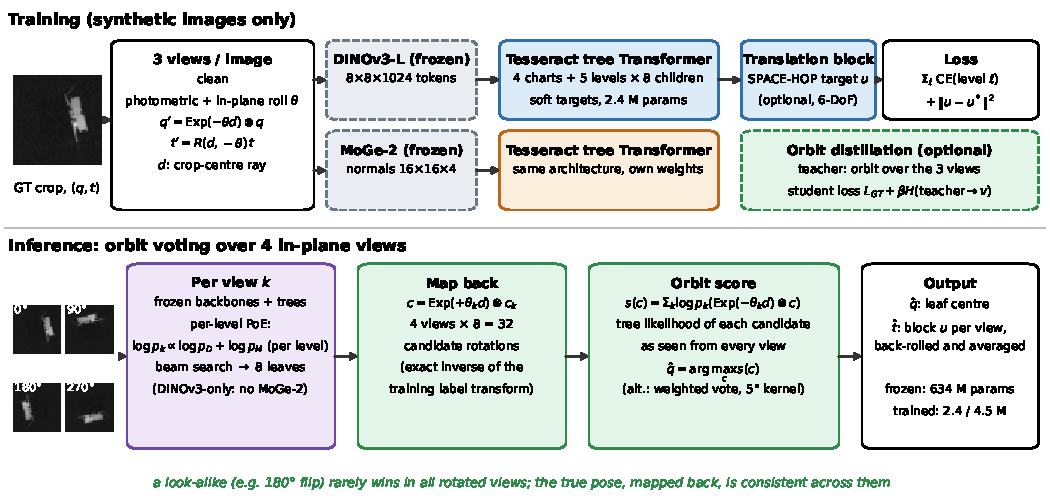
\includegraphics[width=\linewidth]{figures/pipeline.pdf}
  \caption{\textbf{Overview.} \emph{Top:} training. Each synthetic crop is used as a clean view and as two augmented copies (photometric augmentation plus an in-plane roll $\theta$ with exactly transformed labels). Frozen DINOv3 and MoGe-2 features feed one tesseract tree Transformer each; an optional translation block reads the same tokens, and optional orbit distillation replaces the ground-truth target by an orbit teacher. \emph{Bottom:} orbit voting at test time. Candidates from four rotated views are mapped back to a common frame and scored by their per-level PoE tree likelihood in every view.}
  \label{fig:pipeline}
\end{figure*}

\Cref{fig:pipeline} gives an overview of training and inference.

\subsection{Problem setup}
Given a square crop of a known object around its bounding box (15\% margin per side), we predict the rotation $q\in SO(3)$ (unit quaternion, $q\equiv-q$) of the object frame relative to the camera and the translation $t\in\mathbb{R}^3$. For objects that appear away from the optical axis (T-LESS, YCB-V), the tree predicts the \emph{allocentric} rotation $R_{\text{ray}}(t)^\top R$, which removes the viewing-ray component so that the crop's appearance depends only on the predicted rotation; it is converted back exactly. Rotation error is $E_R=2\arccos|\langle\hat q,q\rangle|$, minimised over the object's symmetry set $\mathcal{S}$ when one exists ($\min_{S\in\mathcal{S}} E_R(\hat q, q\,S)$), and translation error is $E_T=\|\hat t-t\|_2$.

\subsection{Tesseract tree on $SO(3)$}
\label{sec:tree}
Following the recursive tesseract subdivision~\cite{kurz2017tesseract}, a quaternion is assigned to a \emph{chart} $c=\arg\max_i|q_i|$, sign-normalised so that $q_c>0$ (this identifies $q$ and $-q$), and projected to the cube $x=q/q_c$. Its three free coordinates in $[-1,1]$ are halved recursively, so each level selects one of 8 children.
We use \emph{cell centres} (lifted back to the unit sphere) as representatives. Unlike corner representatives, every rotation then has a unique root-to-leaf path. With 4 charts and depth 5 there are $4\cdot 8^5=131{,}072$ cells. The quantisation error of the leaf centre is $2.51^\circ$ on average ($3.97^\circ$ p95, $6.20^\circ$ worst case), and it halves per level. For objects without symmetry this floor bounds the fine accuracy of our rotation results; for symmetric objects the nearest leaf to \emph{any} equivalent rotation is closer.

\paragraph{Tree Transformer.}
For each backbone, a small decoder predicts the path autoregressively. The frozen tokens are layer-normalised, linearly projected to $d=256$, given 2-D positional encodings and passed through one encoder layer. A causal decoder with 2 layers (4 heads, FFN 512) then reads a sequence that starts with a root token followed by one token per decided level. Each such token embeds the level and a 6-frequency Fourier encoding of the current cell centre, and cross-attends to the encoded image tokens. The root position predicts the chart (4 logits) and position $\ell$ predicts the child (8 logits). The model has 2.4\,M parameters.
We train with geodesic soft targets: at each level, the target over the candidate cells is $\propto\exp(-(\delta/\tau_\ell)^2)$, where $\delta$ is the angle between the ground truth and each cell centre. The widths $\tau_\ell$ ($39.3^\circ$ for the root and level 1, $20.0^\circ$, $10.0^\circ$, $5.0^\circ$, $2.5^\circ$) halve with the cell size. Training uses teacher forcing on the ground-truth path and a cross-entropy at every level; inference is greedy or beam search, and the prediction is the leaf centre.

\paragraph{Frozen features.}
DINOv3 ViT-L/16~\cite{simeoni2025dinov3} last-layer patch tokens are average-pooled to an $8{\times}8$ grid ($64\times1024$). For geometry, MoGe-2~\cite{wang2025moge2} surface normals are masked by a foreground mask on which both backbones agree (the intersection of a DINOv3 foreground estimate and the MoGe-2 mask). They are then pooled to $16{\times}16$ cells, each holding three masked-normal channels and the mask fraction ($256\times4$). This consensus mask removes most of MoGe-2's background leakage on real images (\cref{sec:supp_lineage}). Features are extracted once; only the trees are trained.

\paragraph{Per-level product of experts.}
The two trees are fused without training. At every decoding step, the log-softmax distributions of both branches are added and renormalised: $\log p^{(\ell)}\propto\log p^{(\ell)}_{\text{DINO}}+\log p^{(\ell)}_{\text{MoGe}}$. Beam search then runs on the fused tree. We report this \emph{PoE} variant and a faster \emph{DINOv3-only} variant.

\subsection{Symmetry-aware multi-path targets}
\label{sec:symtarget}
For a symmetric object, the annotated rotation $q$ is one arbitrary member of the equivalence set $\{q\,s : s\in\mathcal{S}\}$, where $\mathcal{S}$ holds the object-frame symmetries (continuous symmetries discretised). Training on $q$ alone (\emph{single label}) gives contradictory targets for identical images. The usual fix maps every label to a \emph{canonical} member, \eg the one closest to identity. This removes the contradiction but makes the target a discontinuous function of the image: two nearly identical views can receive canonical labels far apart, and the in-plane relation of \cref{eq:roll} no longer holds between views.
Instead, we train the tree on all equivalent rotations. The loss is the soft-target cross-entropy of \cref{sec:tree}, averaged over the members of the set, each with teacher forcing along its own path:
\begin{equation}
  \mathcal{L}_{\text{sym}}=\frac{1}{|\mathcal{S}'|}\sum_{s\in\mathcal{S}'}\mathcal{L}_{\text{GT}}\big(q\,s\big),
  \label{eq:symloss}
\end{equation}
where $\mathcal{S}'=\mathcal{S}$ if $|\mathcal{S}|\le 8$ and otherwise 8 members are drawn per sample and step (an unbiased estimate). The tree learns to split its probability between the equivalent paths, which is the level-marginal target of the whole set. For objects without symmetry \cref{eq:symloss} reduces exactly to the standard loss. Right-multiplication by $s$ commutes with the roll of \cref{eq:roll}, so augmented views and orbit voting are unchanged; we verified both identities numerically ($<10^{-9}$).

\subsection{Augmentation with exact in-plane labels}
\label{sec:aug}
Each training image is used as a clean crop and as two pre-extracted augmented copies; one of the three is drawn at every step. The augmentations are photometric (brightness, contrast, gamma, blur, glare blobs, noise, random erasing, JPEG) plus an in-plane rotation of the crop by $\theta\sim\mathcal{U}(-180^\circ,180^\circ)$ about its centre.
Rotating the crop about its centre is equivalent to rotating the camera about the unit ray $d$ through the crop centre, computed with the lens distortion removed. Points therefore transform as $p'=R(d,-\theta)\,p$, and the labels as
\begin{equation}
  q' = \Exp(-\theta\, d)\otimes q,\qquad t'=R(d,-\theta)\,t .
  \label{eq:roll}
\end{equation}
We derived this convention from the camera geometry rather than fitting it to a predictor. Projecting model keypoints with $q'$ reproduces the warped image to $0.2^\circ$ (p95 label error measured by PnP). For datasets whose objects lie far from the optical axis (T-LESS, YCB-V), an affine crop rotation is not exactly a camera roll (label error up to $6.7^\circ$). There we warp with the roll homography $K R(d,-\theta) K^{-1}$ instead, which makes \cref{eq:roll} exact (verified to $0.000^\circ$).

\subsection{Orbit voting}
\label{sec:orbit}
At test time we form $K{=}4$ views of the crop rotated by $\theta_k\in\{0^\circ,90^\circ,180^\circ,270^\circ\}$. In view $k$ the fused tree's beam search returns 8 leaves $c_{k,1..8}$, which are mapped back to the original frame by the inverse of \cref{eq:roll}, $c=\Exp(+\theta_k d)\otimes c_k$, giving 32 candidates. Each candidate $c$ is then scored by the tree likelihood of its own path when mapped into every view:
\begin{equation}
  s(c)=\sum_{k=1}^{K}\log p_k\big(\mathrm{path}(\Exp(-\theta_k d)\otimes c)\big),
  \label{eq:orbit}
\end{equation}
and predict $\hat q=\arg\max_c s(c)$. Here $\log p_k$ sums the fused root and child log-probabilities along the path, evaluated with teacher forcing. A $180^\circ$ look-alike that wins in one view must also be likely in the other three to be selected, whereas the true pose is consistent by construction.
We also evaluate a \emph{weighted vote}, in which each candidate collects Gaussian-kernel support ($5^\circ$) from the other candidates, weighted by their normalised beam probabilities within their view. Orbit voting has no parameters and multiplies inference cost by about $4\times$ (\cref{tab:main}).

\subsection{Orbit distillation}
\label{sec:distill}
Orbit voting is more accurate than a single view, so we use it as a teacher. For every training image we run the frozen orbit system over its three available views (clean and two augmented, with known rolls). This gives 24 candidates in the clean frame with weights $w_j=\mathrm{softmax}_j\, s(c_j)$. A new tree per branch is then trained from scratch with the same recipe and the loss
\begin{equation}
\begin{split}
  \mathcal{L}=\;&\mathcal{L}_{\text{GT}}(v)\\
  &-\frac{\beta}{L{+}1}\sum_j w_j\sum_{\ell=0}^{L}\log p^{(\ell)}\big(\mathrm{pre}_\ell(\Exp(-\theta_v d)\otimes c_j)\big),
\end{split}
  \label{eq:distill}
\end{equation}
with $\beta=1$ and $\mathrm{pre}_\ell$ the length-$\ell$ path prefix. Here $v$ is the view drawn for the image, and the teacher candidates are transported into its frame. The student is a single-view model with unchanged inference cost; at test time it can be used alone or with orbit voting. This is a data-distillation scheme~\cite{radosavovic2018data} applied to hierarchical rotation targets.

\subsection{Translation block (6-DoF)}
\label{sec:sixdof_method}
For translation we keep the SPACE-HOP parameterisation~\cite{dutta2026spacehop} unchanged. With box centre $(b_x,b_y)$ and size $(b_w,b_h)$, image size $(W,H)$, intrinsics $(f_x,f_y,c_x,c_y)$ and $\alpha=1.6$, the target is $u=(U_x,U_y,U_z)$ with
\begin{align}
U_x&=\tfrac{1}{b_w}\big(f_x\tfrac{X}{Z}+c_x-b_x\big),\quad U_y=\tfrac{1}{b_h}\big(f_y\tfrac{Y}{Z}+c_y-b_y\big),\\
U_z&=\tfrac{1}{2}\big(\tfrac{\alpha b_w}{W}+\tfrac{b_h}{H}\big)Z,
\end{align}
trained with $\|u-u^*\|^2$ and inverted in closed form. A translation block (one learned query cross-attending to the tree's encoded tokens, then an MLP) predicts $u$. It is trained either jointly with the tree ($\mathcal{L}_{\text{tree}}+\mathcal{L}_{\text{trans}}$) or on a frozen tree. Rolled views use $t'$ from \cref{eq:roll} with the unchanged box. With orbit voting, each view's $\hat t$ is rolled back and the four are averaged.
